\section{Inductance Chain (6th September 2018)}
 \subsection{On the topic of inductance chain}
  \iframe{The idea is to create a chain of inductors and JJ that would not pass microwaves, \red{because the inductance of the system is $ \le 0 $.}}
  
  We should begin by giving the definition of inductance:
  
  \[
  	E = \frac{\Phi^2}{2L} \ira \frac{1}{L} = \difffrac{E^2}{^2\Phi} = \bigg(\frac{2\pi}{\Phi_0}\bigg)^2\difffrac{E^2}{^2\phi} 
  \]
  
  \ipicCaption{5cm}{inductor_chain}{The combination of the parabollic energy from the inductor and the sinusoidal energy of the JJ will give a very flat energy with resepct to phase. In this saddle $ \difffrac{E^2}{^2\Phi} $, so inductance is infinite.} 
 
  \begin{enumerate}
  	\item We write out the energy of the JJ and the inductor and remember the quantisation condition in a loop:
  	\[
  		\ialigned{
  			E_J & = - E_{J0}\cos(\phi_{JJ}) \qquad\red{1-\cos(\phi_{JJ})};\\
  			E_L & = \left(\frac{\Phi_0}{2\pi}\right)^2\frac{\phi_L^2}{2L}\\
  			2\pi n & = \phi_{JJ} + \phi_{L} + \phi_{ext}
  		} \iratext{n=0}
  		E = -E_{J0}\cos(\phi_{JJ}); + E_{L0}\frac{(\phi_{ext} + \phi_{L} )^2}{2L}
  	\]
  	\item We have another condition, in that the current circulating in the loop must be the same for both the JJ and for the inductor:
  	\[
  		\ialigned{
  			I & = I_0\sin(\phi_{JJ})\\
  			I & = \frac{\Phi_{ext}}{L} = \frac{\Phi_0}{2\pi}\frac{\phi_{ext}}{L}
  		} \iRa
  		\sin(\phi_{JJ}) = \frac{\Phi_0}{2\pi I_0}\frac{\phi_{ext}}{L}
  	\]
  	\item Combining the above equations and finding the inductance of the full system:
  	\begin{equation}\label{eqn:6sep_1}
  		\ialigned{\frac{1}{L_{\text{full}}} = \bigg(\frac{2\pi}{\Phi_0}\bigg)^2\difffrac{E^2}{^2\phi}  = \bigg(\frac{2\pi}{\Phi_0}\bigg)^2\difffrac{^2}{^2\phi_{ext}}\bigg[-E_{J0}\sqrt{1-\bigg(\frac{\Phi_0\phi_{ext}}{2\pi I_0 L}\bigg)^2} + \left(\frac{\Phi_0}{2\pi}\right)^2\frac{(\phi_{ext} + \phi_{L} )^2}{2L}\bigg]\\
  		 = 
  		}
  	\end{equation}
  	\noindent which solves to give a potential $ L_{\text{full}} = \infty $.
  \end{enumerate}

 \subsection{On the topic of my stalling PhD}
  The discussion revolved around resonators and our ability to tune their frequency. We have seen in Eq.~\eqref{eqn:6sep_1} that we can change the inductance of our resonator.
  
  Because the speed of a microwave through a system with inductance and capacitance per unit length $ l $ and $ c $ respectively
  
  \[
  	v = \frac{1}{lc},
  \]

  \noindent and the frequency of the resonator
  
  \[
  	T = \frac{a}{v}\times 2 \ra f = \frac{1}{2a\sqrt{lc}}.
  \]
  
  \noindent For a \iunit{10}{GHz} resonator, we need a length, $ a $, of:
  
  \[
  	a \approx \frac{1}{2a\sqrt{\mu_0}\epsilon_0} \approx \iunit{1.5}{mm}.
  \]
  
  \subsection{Interesting fabrication techniques}
   \begin{itemize}
   	\item When making a resonator and ground planes, etch out the dielectric that is in the gap between them. This way the resonator cannot leak to the ground plane through the substrate;
   	\item Treat substrate with HF to remove oxide and only then deposit niobium or aluminium.
   \end{itemize}
  \subsection{What is in it for me}
   The system of a qubit integrated into a resonator has been studied previously: matching the frequency of the qubit to the frequency of the resonator, creates a interacting ladder state, where the resonator-qubit system splits into two energies. 
   
   \ipic{4cm}{ladder}
  
   \noindent The output spectrum will therefore have two peaks 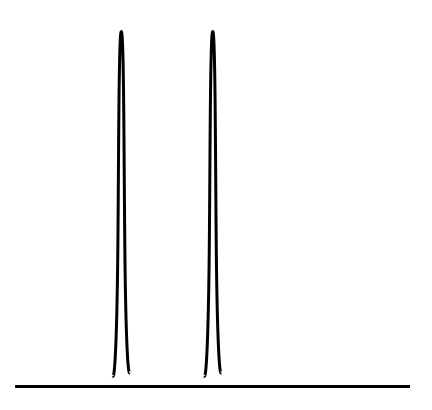
\includegraphics[height=3cm]{res_2peak}.
   
   What if we flip this case and use the qubit as the system for reading out? Consider the two cases below.
   
   \ipic{5cm}{06sep_2}
   
   In the second case we use a resonator, which has infinitely many modes, that will be effecting the state of the qubit. \red{For each of the two qubit states, \iket{0} and \iket{1}, there will be an infinte number of resonator modes that will be shifting its energy for readout which we do with the tranmission line}:
   
   \ipic{5cm}{6sep_1}
   
   So now at the output, the qubit will be emitting a spectum of energies:
   
   \ipic{3cm}{6sep_03}
   
  
